\section{Adaption of Business Process Management}
\label{sec:bpm}
After having introduced microservices and their event-based choreography we now take \acrfull{bpm} into account. This technique gains relevance when trying to set up the data warehousing process to be as adaptive as possible. Furthermore, it will enable one to overcome the challenges pointed out while talking about the event-based microservice architecture.\newline
First of all, the term BPM will be defined in regard to Data Warehouse Systems. Based on this foundation, the process-driven approach can be introduced. 

\subsection{Defining Business Process Management}
''\acrfull{bpm} is a systemic approach geared to capture, design, execute, document, measure, monitor and control automated as well as non-automated processes in order to meet the objectives that are aligned with the business strategy of a company.'' \cite{bpmDef} Another important aspect is BPM trying to focus on end-to-end processes. This means that processes are considered as whole without any separation into fragments. \cite{praxisBPM}\newline
\\
In order to provide uniform processes and make them generally interpretative, the \acrfull{omg} defined the \acrfull{bpmn} standard which is currently in its second version. A positive aspect of this is that the standard isn't owned or controlled by any company and can be used for free in various tools. In contrast to workflow tools there won't be any problems by switching the BPM tooling due to this standardisation. \cite{bpmMethodStyle}

\subsection{Applying BPM to the Data Warehousing Process}
In this section, we consider the data warehousing process which was introduced in chapter \ref{sec:referenceArchitecture} as an end-to-end process. The corresponding BPMN model can be found in figure \ref{fig:BPMNdatawarehousing}.\newline
By having the tasks surrounded by the process pool, the context of the data warehousing process is defined. BPMN offers various start events. In this case a cyclic timer was chosen to start the whole process. Afterwards cascading calling tasks can be seen which encapsulate various sub-processes. In the end the process terminates successfully. In this simple example, it was decided to explicitly not use any kind of error handling to reduce its complexity.\newline
\begin{figure}[!htb]
    \centering
    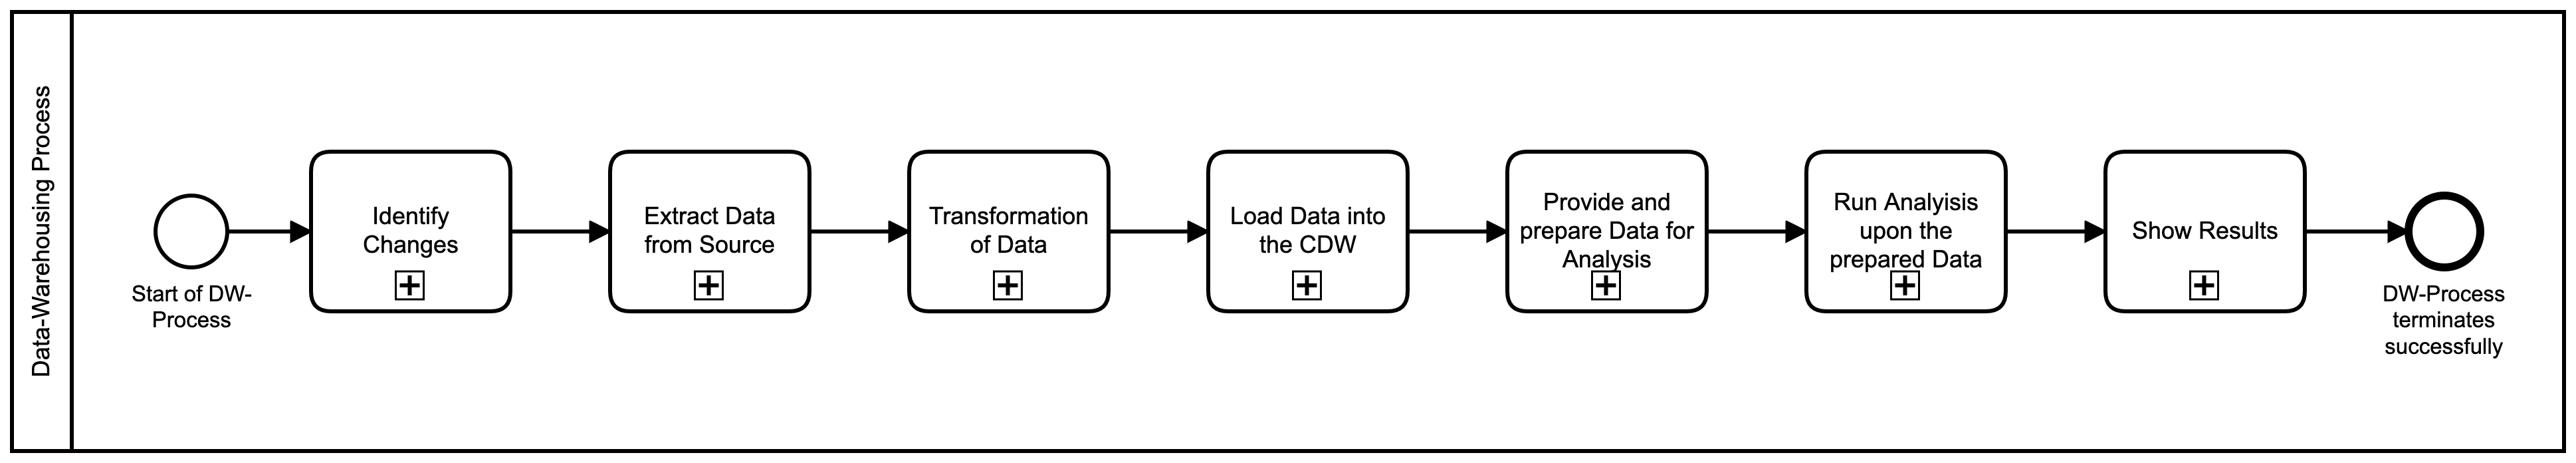
\includegraphics[scale=0.15]{pictures/DataWarehousingProcess.png}
    \caption{BPMN 2.0 visualisation of the data warehousing process}
    \label{fig:BPMNdatawarehousing}
\end{figure}\\
Figure \ref{fig:BPMNdatatransformation} shows a sub-process called from its parent diagram (figure \ref{fig:BPMNdatawarehousing}) in more detail. Of course, this is just an example that can be adapted. By using this example, the purpose and benefits of BPM in data warehouse systems get more obvious.\newline
As shown in the data transformation process, it is possible to cascade multiple tasks with each other. Having automated as well as non-automated user tasks will not require a split within the process flow. It is also possible to make decisions based on the result of previous tasks. Due to this, the creation and adaption of data warehouse processes with BPMN 2.0 is quite smooth. It easily can be thought of having separated case distinctions for various department needs or how to react on different input formats.\newline 
The three vertical lines beneath some of those tasks indicate that a multi-instance task is given. ''It allows execution of a certain step or even a complete sub process for each item in a given collection, [...] in parallel.'' \cite{bpmMultiInstance} \newline
\begin{figure}[!htb]
    \centering
    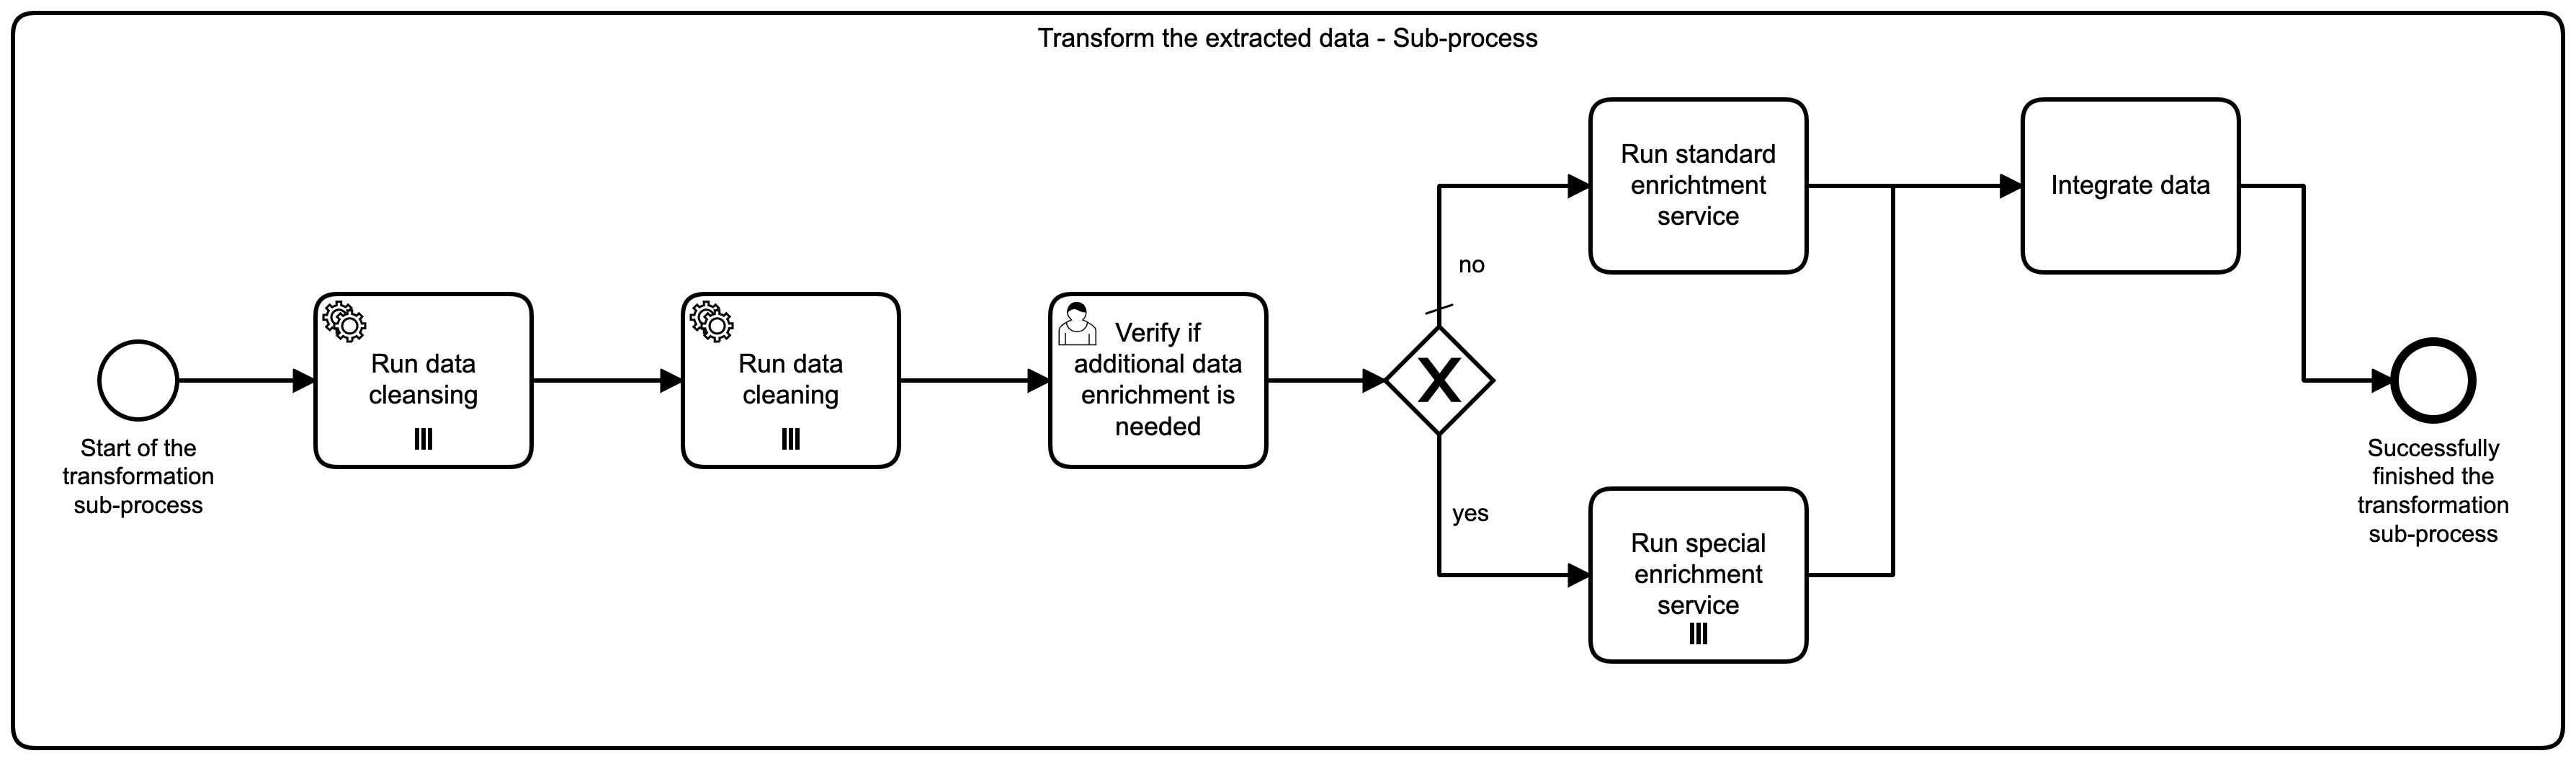
\includegraphics[scale=0.13]{pictures/DataTransformationSubprocess.png}
    \caption{BPMN 2.0 visualisation of a possible sub process for data transformation}
    \label{fig:BPMNdatatransformation}
\end{figure}
\\
In the next chapter the introduced know-how concerning BPM will be used as a way to orchestrate microservices. This will result in the process driven architecture which will be crucial to the resulting DWS architecture.

\subsection{Resulting Process-Driven Approach and its Advantages}
Next up, it will be shown how BPM can be used to orchestrate microservices and especially self-contained systems. The aim of this integration is to have a more adaptive microservice landscape, which can be used within our DWS. As the basis for our discussion we will make use of the challenges of event-based microservice choreography introduced in chapter \ref{sec:eventBasedArchitecture}.\newline
\\
\\
By choosing the approach that contains a workflow engine used for orchestrating REST calls by Bernd Rücker, it is possible to achieve the previously introduced goal. The workflow engine itself is used for running processes written in BPMN. Additional details about the corresponding implementation can be linked within this notation as well.\newline
In his blog post ''The Microservices Workflow Automation Cheat Sheet'' Bernd Rücker introduced this architecture with an example of an order which separates into services such as checkout, payment and shipment. Via the workflow engine those can be linked as shown in figure \ref{fig:RestArchitecture}. \cite{orchestrationMicroServices}\newline
\begin{figure}[!htb]
    \centering
    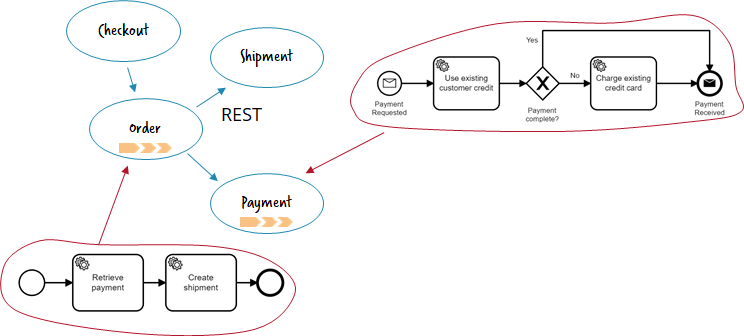
\includegraphics[scale=0.65]{pictures/RestArchitecture.png}
    \caption{Point-to-point communication by request/response \cite{orchestrationMicroServices}}
    \label{fig:RestArchitecture}
\end{figure}
This architecture makes use of REST to call other microservices in a synchronous way. As seen, the workflow engine can be contained within one or multiple microservices. \cite{orchestrationMicroServices} Typically, the overall process is stored within the meta-service ''Order'' summarising the purpose of the system. By making use of multiple workflow engines within the services it is possible to apply this concept to called services as well. Due to this the ''Payment'' service can also be replaced by a cluster of multiple services which are orchestrated by the overall payment service.\newline
To sum up the purpose of the workflow engine in this architecture Rücker states the following: ''stateful resilience patterns (like stateful retry), timeout handling, managing activity chains / the flow, consistency and compensation handling aka Saga pattern [...].'' \cite{orchestrationMicroServices}\newline
\\
By having a look back on the challenges from the event-based bus architecture, we now analyse if this approach provides any benefits. \\
\begin{itemize}
    \item ''Flow of events'': By having an orchestrated approach it is always defined how the events / tokens flow through the system. Additionally, most of the engines provide historic information about all tokens which have travelled through the process. Due to this, the behaviour is always reproducible and compliant. 
    \item ''Losing sight of flow'': Since the BPMN model guides through the flow and is well-defined, this issue won't occur within this approach.
    \item ''SLAs and resilience'': Since the engine's purpose is to act within a stateful resilience pattern, this challenge has been solved as well. Nevertheless, having the overall process contained in one service means that a single point of failure can exist. 
    \item ''Wired coupling'': If a new service will be added within the process, it will only affect its parent. By adding an ''Age Check'' to our order process all adaptions would be contained within the process definition of the ''Order'' parent service. No other services will be affected. Due to this wired coupling is rarer than within event-based systems. A negative is that a stateful \acrshort{rest} connection is chosen instead of an asynchronous possibility which is emphasised by the SCS's architectural approach. 
\end{itemize}
Overall, it can be seen that the usage of a process driven architecture in order to orchestrate microservices can be beneficial. This technique will further result in a concrete data warehouse architecture which will be introduced in the next chapter. 
